\documentclass[12pt,a4paper]{article}
\usepackage[polish]{babel}
\usepackage[T1]{fontenc}
\usepackage[]{algorithm2e}
\usepackage{listings}

\usepackage{color}
\usepackage{listings}

\usepackage{graphicx}
\usepackage{wrapfig}
\usepackage{dirtree}
\usepackage{tikz}
\usetikzlibrary{shapes.geometric,arrows,positioning,calc}

\lstloadlanguages{% Check Dokumentation for further languages ...
	C,
	C++,
	csh,
	Java
}

\definecolor{red}{rgb}{0.6,0,0} % for strings
\definecolor{blue}{rgb}{0,0,0.6}
\definecolor{green}{rgb}{0,0.8,0}
\definecolor{cyan}{rgb}{0.0,0.6,0.6}

\lstset{
	language=csh,
	basicstyle=\footnotesize\ttfamily,
	numbers=left,
	numberstyle=\tiny,
	numbersep=5pt,
	tabsize=2,
	extendedchars=true,
	breaklines=true,
	frame=b,
	stringstyle=\color{blue}\ttfamily,
	showspaces=false,
	showtabs=false,
	xleftmargin=17pt,
	framexleftmargin=17pt,
	framexrightmargin=5pt,
	framexbottommargin=4pt,
	commentstyle=\color{green},
	morecomment=[l]{//}, %use comment-line-style!
	morecomment=[s]{/*}{*/}, %for multiline comments
	showstringspaces=false,
	morekeywords={ abstract, event, new, struct,
		as, explicit, null, switch,
		base, extern, object, this,
		bool, false, operator, throw,
		break, finally, out, true,
		byte, fixed, override, try,
		case, float, params, typeof,
		catch, for, private, uint,
		char, foreach, protected, ulong,
		checked, goto, public, unchecked,
		class, if, readonly, unsafe,
		const, implicit, ref, ushort,
		continue, in, return, using,
		decimal, int, sbyte, virtual,
		default, interface, sealed, volatile,
		delegate, internal, short, void,
		do, is, sizeof, while,
		double, lock, stackalloc,
		else, long, static,
		enum, namespace, string},
	keywordstyle=\color{cyan},
	identifierstyle=\color{red},
    literate={♠}{{$\spadesuit$}}1 {♣}{{$\clubsuit$}}1 {♦}{{$\diamondsuit$}}1 {♥}{{$\heartsuit$}}1
}

\usepackage{caption}
\DeclareCaptionFont{white}{\color{white}}
\DeclareCaptionFormat{listing}{\colorbox{blue}{\parbox{\textwidth}{\hspace{15pt}#1#2#3}}}
\captionsetup[lstlisting]{format=listing,labelfont=white,textfont=white, singlelinecheck=false, margin=0pt, font={bf,footnotesize}}


\addtolength{\hoffset}{-1.5cm}
\addtolength{\marginparwidth}{-1.5cm}
\addtolength{\textwidth}{3cm}
\addtolength{\voffset}{-1cm}
\addtolength{\textheight}{2.5cm}
\setlength{\topmargin}{0cm}
\setlength{\headheight}{0cm}

\tikzstyle{startstop} = [rectangle, rounded corners, minimum width = 3cm, minimum height = 1cm, text centered, text width = 2.5cm, draw = black]
\tikzstyle{io} = [trapezium, trapezium left angle = 70, trapezium right angle = 110, minimum width = 3cm, minimum height = 1cm, text centered, text width = 2.5cm, draw = black]
\tikzstyle{process} = [rectangle, minimum width = 3cm, minimum height = 1cm, text centered, text width = 2.5cm, draw = black]
\tikzstyle{decision} = [diamond, aspect = 3, minimum width = 3cm, minimum height = 1cm, text centered, text width = 3cm, draw = black]
\tikzstyle{arrow} = [thick, ->, > = stealth]

\makeatletter
\pgfdeclareshape{datastore}{
  \inheritsavedanchors[from=rectangle]
  \inheritanchorborder[from=rectangle]
  \inheritanchor[from=rectangle]{center}
  \inheritanchor[from=rectangle]{base}
  \inheritanchor[from=rectangle]{north}
  \inheritanchor[from=rectangle]{north east}
  \inheritanchor[from=rectangle]{east}
  \inheritanchor[from=rectangle]{south east}
  \inheritanchor[from=rectangle]{south}
  \inheritanchor[from=rectangle]{south west}
  \inheritanchor[from=rectangle]{west}
  \inheritanchor[from=rectangle]{north west}
  \backgroundpath{
    %  store lower right in xa/ya and upper right in xb/yb
    \southwest \pgf@xa=\pgf@x \pgf@ya=\pgf@y
    \northeast \pgf@xb=\pgf@x \pgf@yb=\pgf@y
    \pgfpathmoveto{\pgfpoint{\pgf@xa}{\pgf@ya}}
    \pgfpathlineto{\pgfpoint{\pgf@xb}{\pgf@ya}}
    \pgfpathmoveto{\pgfpoint{\pgf@xa}{\pgf@yb}}
    \pgfpathlineto{\pgfpoint{\pgf@xb}{\pgf@yb}}
 }
}
\makeatother

\begin{document}
	
\title{Języki skryptowe\\\small{dokumentacja projektu Pasjans}}
\author{Karolina Kozubik\\grupa 3/5, Informatyka st. I, rok II\\Wydział Matematyki Stosowanej}
\date{\today}

\maketitle
\newpage
\section*{Część I}
\subsection*{Opis programu}
Celem projektu było zaproponowanie infrastruktury serwerowej realizującej Zadanie 5 z konkursu Algorytmion z roku 2016. Pełna treść zadania:

Pasjans jest grą karcianą (najczęściej jednoosobową), której celem jest ułożenie krat wg pewnego wzorca. W zdecydowanej większości pasjansów powodzenie gracza zależy od jego umiejętności, istnieje jednak i taki, który zależy tylko od „szczęścia” gracza. W pasjansie tym, po przetasowaniu talii 24 krat, układamy (koszulkami do góry) cztery rzędy krat po sześć – z wyjątkiem rzędu czwartego, w którym ostatnią kartę zatrzymujemy w dłoni. Celem gry jest ułożenie kart we właściwej kolejności: w pierwszym rzędzie kiery (9, 10, walet, dama, król i as), w kolejnych odpowiednie kolory to: karo, trefl i pik (kolejność figur jak w kierach). Gra kończy się, gdy w dłoni mieć będziemy asa pik. Jeśli kartą w dłoni nie jest as pik, to kładziemy ją (obrazkiem do góry) na odpowiadające jej miejsce (np. gdyby była to dama tref, to odłożylibyśmy ją do rzędu trzeciego do czwartej kolumny), biorąc w dłoń leżącą tam kartę. Jeśli natrafimy ostatecznie na asa pik, to (o ile będzie taka potrzeba) odsłaniamy, nie zmieniając ich położeń w układzie, pozostałe nieodsłonięte (leżące koszulkami do góry) dotychczas karty. Jeżeli wszystkie karty leżeć będą we właściwej kolejności – wygraliśmy, jeśli nie – przegraliśmy. Napisz program, który generował będzie losowe rozłożenie kart, a następnie rozgrywał będzie partie tego pasjansa. Program działał będzie do pierwszego zwycięstwa. Partie przegrane nie interesują nas, chcemy jedynie wiedzieć, za którym razem wygraliśmy oraz zobaczyć wizualizację zwycięskiej partii. Przez wizualizację rozumiemy tutaj kolejne ruchy gracza począwszy od wejściowego układu, a skończywszy na asie pik „w dłoni” (łącznie z ewentualnym odsłanianiem kart nieodsłoniętych). Sposób tej wizualizacji pozostawiamy w gestii rozwiązującego. \cite{algorytmion}

W celu spełnienia założeń projektu, zadanie zostało zmodyfikowane. Algorytm przyjmuje liczbę oznaczającą ilość partii, jaką może maksymalnie rozegrać. Algorytm kończy działanie, jeśli rozegra daną ilość partii lub wcześniej, jeśli rozegrana partia zakończy się sukcesem. Algorytm zwraca liczbę faktycznie rozegranych partii, informację o tym, czy udało się wygrać, oraz reprezentację ostatniej rozegranej partii.

Program zarządzający realizacją algorytmu pobiera dane wejściowe z katalogu \texttt{/in/}, a dane wyjściowe zapisuje w katalogu \texttt{/out/}. Program po podaniu odpowiednich opcji ma możliwość wygenerowania raportu w pliku \texttt{html}, oraz stworzenia zapasowej kopii raportu opatrzonej znacznikiem czasowym.

\newpage

\subsection*{Instrukcja obsługi}
Program jest wzorowany na aplikacjach konsolowych systemów typu Unix. Aby uruchomić program należy z poziomu konsoli systemowej wykonać skrypt \texttt{run.sh}. Aby uzyskać więcej informacji o programie, należy jako argument podać opcję \texttt{-h} lub \texttt{-{}-help}.

\begin{figure}[h]
    \centering
    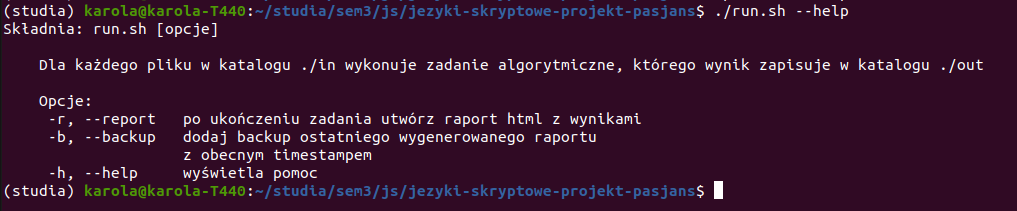
\includegraphics[width=0.75\linewidth]{program-help.png}
    \caption{Uruchomienie programu z opcją -{}-help}
    \label{fig:program-help}
\end{figure}

Program wypisuje na wyjście składnię polecenia oraz opisy opcji, z których można skorzystać. 

Przy podaniu opcji \texttt{-r} lub \texttt{-{}-report} w katalogu \texttt{/report/} tworzony jest plik \texttt{index.html}, który automatycznie otwierany jest w przeglądarce internetowej.

\begin{figure}[h]
    \centering
    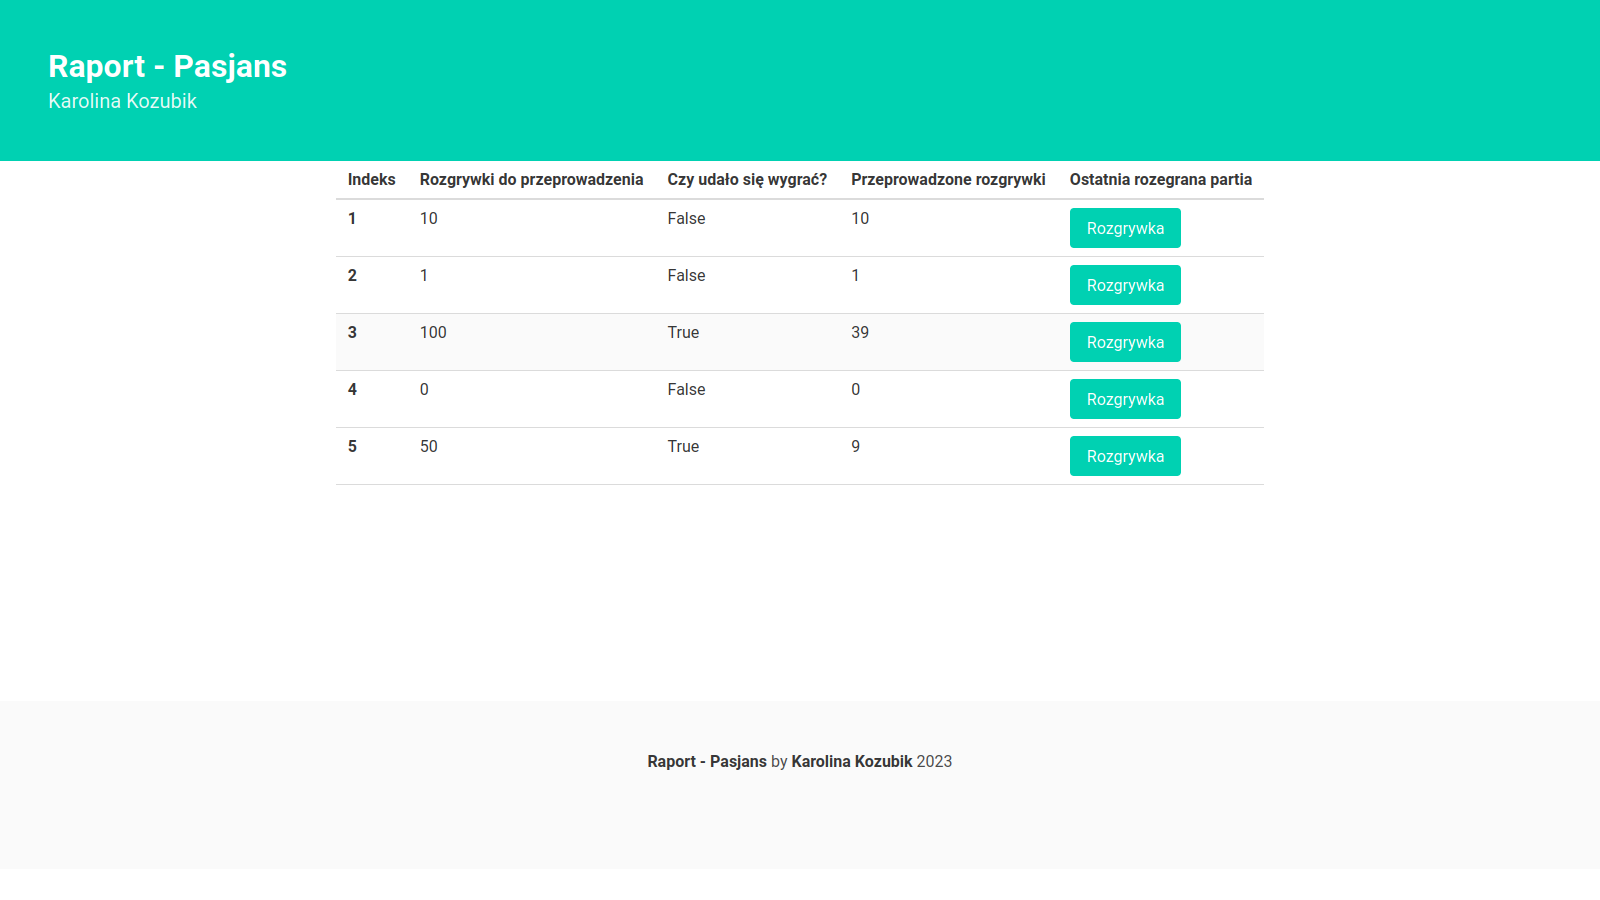
\includegraphics[width=0.75\linewidth]{raport.png}
    \caption{Wygenerowany raport}
    \label{fig:raport}
\end{figure}

W raporcie prezentowana jest tabela informująca o przebiegu programu dla kolejnych danych wejściowych. W kolumnie \texttt{Rozgrywki do przeprowadzenia} widoczne są dane wejściowe dla programu. Następnie program informuje, czy udało się wygrać oraz ile faktycznie rozgrywek przeprowadzono. Ostatnia kolumna zawiera przycisk umożliwiający rozwinięcie wizualizacji ostatniej rozegranej w danym przebiegu partii.

Za każdym razem, gdy nie udało się osiągnąć zwycięstwa, liczba przeprowadzonych partii nie będzie się różniła od ilości partii zadanych do rozegrania. Jednak gdy wykonanie programu zakończyło się wcześniej ze względu na wygraną rozgrywkę, jesteśmy w stanie ustalić, jak szybko to nastąpiło.

\begin{figure}
    \centering
    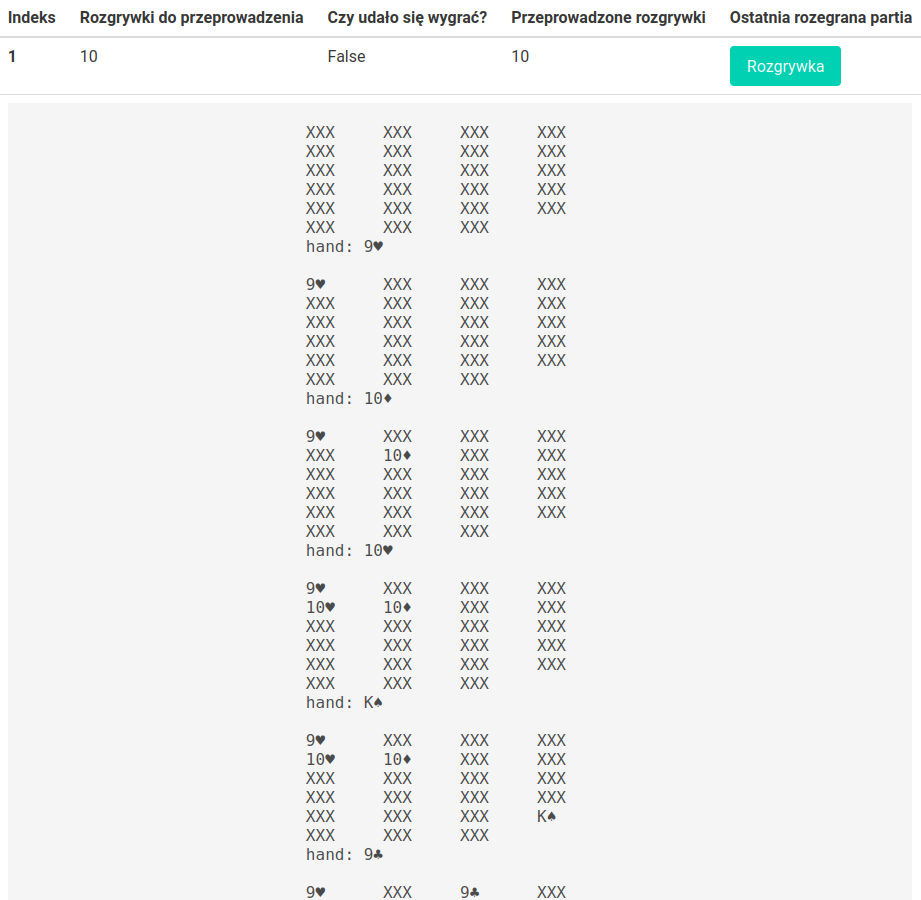
\includegraphics[width=0.75\linewidth]{raport-rozgrywka.png}
    \caption{Widok rozgrywki w raporcie}
    \label{fig:report-game}
\end{figure}

\begin{wrapfigure}{r}{0.4\textwidth}
    \centering
    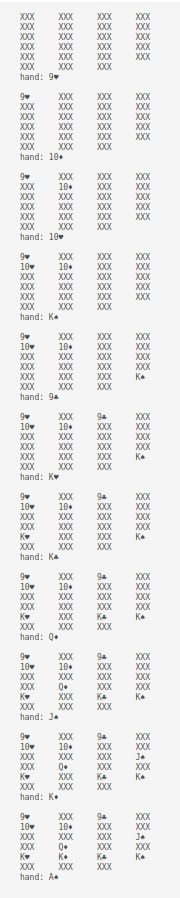
\includegraphics[width=0.6\linewidth]{pelna-rozgrywka.png}
    \vspace{-15.0pt}
    \caption{Pełna rozgrywka}
    \label{fig:full-game}
\end{wrapfigure}


Reprezentacja rozgrywki zawiera kolejne układy planszy. Każda karta na planszy jest reprezentowana odpowiadającym jej symbolem, lub ciągiem \texttt{XXX}, w przypadku, gdy karta jest zasłonięta. Układ pokazuje cztery kolumny po 6 kart, oraz kartę obecnie znajdującą się na ręce. Każda kolejna plansza reprezentuje układ powstały po podmianie karty z ręki z odpowiadającą jej pozycji kartą z planszy. W przypadku, gdy rozgrywka zakończona jest niepowodzeniem, ostatnia plansza nie wskazuje wszystkich odsłoniętych kart, a jedynie te, które udało się odwrócić w czasie gry.

Ostatnią dostępną w programie opcją jest \texttt{-b} lub \texttt{-{}-backup}, która odpowiada za generowanie kopii zapasowej raportu opatrzonej znacznikiem czasowym. Przykładowy wygenerowany w ten sposób plik może nazywać się:\\ \texttt{backup-2024-01-20T17-58-31-663963.html}

Zawarty w nazwie znacznik czasowy jest reprezentacją obecnej daty oraz czasu w formacie ISO, ze wszystkimi znakami interpunkcyjnymi zastąpionymi myślnikami.

Utworzony w ten sposób plik zawiera również oznaczenie czasowe w nagłówku raportu.

Opcje można dowolnie łączyć, a kolejność ich wykonania zależy od kolejności pojawienia się w linii polecenia.

\subsection*{Dodatkowe informacje}
Do wygenerowania raportu wykorzystano bibliotekę \texttt{jinja2}, która pozwala na wstawianie zmiennych do przygotowanego szablonu z poziomu programu języka Python. Szablon ten znajduje się w pliku \texttt{index.html} w katalogu \texttt{template}.

Raport korzysta z technologii HTML5, JavaScript oraz Bulma CSS. Napisany w JavaScript skrypt zawarty w pliku raportu umożliwia rozwijanie oraz ukrywanie rozgrywek, co zapewnia jednolitość oraz spójność tabeli i wygodę w przeglądaniu danych. Bulma CSS to pakiet służący do stylowania elementów HTML za pomocą klas, co zapewnia estetyczność raportu.

\begin{figure}
    \centering
    
\includegraphics[width=0.75\linewidth]{raport-backup.png}
    \caption{Znacznik czasowy w nagłówku raportu}
    \label{fig:backup-report}
\end{figure}

\newpage

\section*{Część II}
\subsection*{Opis działania} 
Jak ujęto w treści zadania, zwycięstwo w zaproponowanym pasjansie zależy jedynie od losowego ułożenia talii. 

Talia używana w grze składa się z 24 kart. Istnieje $24!$, a zatem $6,20448402 \cdot 10^{23}$ sposobów ułożenia takiej talii.

Prawdopodobieństwo zwycięstwa równa się prawdopodobieństwu dobierania kolejnych kart w taki sposób, aby nie był to as pik. W przypadku dobierania pierwszej karty mamy możliwość dobrania jednej z 24 kart, z których 23 nie są asem pik. Następnie musimy dobrać jedną z pozostałych 23 kart, z których 22 nie są asem pik. W ten sposób możemy obliczyć prawdopodobieństwo zwyciężenia rozgrywki:

\begin{equation}
    \frac{23}{24} \cdot \frac{22}{23} \cdot \frac{21}{22} \cdot ... \cdot \frac{1}{2} = \frac{23!}{24!} \approx  0,04166666667
\end{equation}

Zatem prawdopodobieństwo wygranej wynosi około 4\%.
	
\subsection*{Algorytmy}
Algorytm działa w pętli kończącej się po rozegraniu zadanej ilości rozgrywek lub zwyciężeniu partii. W każdym przebiegu pętli inicjowany jest obiekt klasy \texttt{Game}. Inicjalizacja ta pociąga za sobą inicjalizację obiektów klasy \texttt{Board}, następnie klasy \texttt{Deck}. W czasie inicjalizacji obiektu klasy \texttt{Deck} (talii) tworzone są 24 różne karty (obiekty klasy \texttt{Card}), układane w sposób losowy. Wewnątrz konstruktora klasy \texttt{Board} karty te rozkładane są w dwuwymiarowej tablicy reprezentującej planszę. Po inicjalizacji wszystkich obiektów następuje rozegranie partii. 

Rozgrywka odbywa się w pętli zakańczanej, gdy kartą na ręce jest as pik. Wewnątrz pętli karta z ręki podmieniana jest na odpowiadającą jej pozycji kartę z planszy. Następnie w obiekcie zapisywana jest wizualizacji obecnego stanu planszy.

Po zakończeniu rozgrywki ustalany jest jej wynik. Na sam koniec na wyjście standardowe wypisywana jest reprezentacja ostatniej rozegranej partii, ilość przeprowadzonych rozgrywek oraz informacja o tym, czy udało się wygrać.

\begin{tikzpicture}[node distance = 1.5cm, scale=0.7, every node/.style={scale=0.7}]
    ]
    \node (start) [startstop] {Start};
    \node (n) [process, below of=start] {odczytaj n};
    \node (counter) [process, below of=n] {inicjuj \texttt{counter}};
    \node (game) [process, below of=counter] {inicjuj \texttt{game}};
    \node (result) [decision, below of=game, yshift=-0.5cm] {wygrana lub n-ta rozgrywka?};
    \node (out-counter) [io, left of=result, xshift=-5.25cm] {wypisz counter};
    \node (out-viz) [io, below of=out-counter, text width=3cm] {wypisz\\ wygraną partię};
    \node (out-result) [io, below of=out-viz] {wypisz wynik rozgrywki};
    \node (stop) [startstop, below of=out-result] {Stop};

    \node (counter-plus) [process, right of=result, xshift=4cm] {zwiększ \texttt{counter} o 1};
    \node (new-game) [process, below of=counter-plus] {\texttt{game} = nowa rozgrywka};
    \node (as-pik) [decision, below of=new-game, yshift=-1cm] {czy na ręce jest as pik?};
    \node (replace) [process, right of=as-pik, xshift=4cm] {zamień kartę z ręki z odpowiednią kartą na planszy};
    \node (viz-start) [process, below of=replace, yshift=-2cm] {zapisz reprezentację obecnej planszy};

    \draw [arrow] (start) -- (n);
    \draw [arrow] (n) -- (counter);
    \draw [arrow] (counter) -- (game);
    \draw [arrow] (game) -- (result);
    \draw [arrow] (result) -- node [anchor=south] {tak} (out-counter);
    \draw [arrow] (out-counter) -- (out-viz);
    \draw [arrow] (out-viz) -- (out-result);
    \draw [arrow] (out-result) -- (stop);

    \draw [arrow] (result) -- node [anchor=south] {nie} (counter-plus);
    \draw [arrow] (counter-plus) -- (new-game);
    \draw [arrow] (new-game) -- (as-pik);
    \draw [arrow] (as-pik) -- node [anchor=south] {nie} (replace);
    \draw [arrow] (replace) -- (viz-start);
    \draw [arrow] (viz-start) -| (as-pik);

    \draw [arrow] (as-pik) -| node [anchor=south west] {tak} (result);
\end{tikzpicture}

\newpage

\subsection*{Implementacja systemu}
% Opis, zasada i działanie programu ze względu na podział na pliki, nastepnie	funkcje programu wraz ze szczegółowym opisem działania (np.: formie pseudokodu, czy odniesienia do równania)
% \begin{lstlisting}
% 	Tutaj wklejamy fragment kodu, ktory chcemy opisac 
% 	(bez polskich znakow).
% \end{lstlisting}

Struktura programu wygląda następująco:
\dirtree{%
.1 /.
.2 main.py.
.2 app.
.3 Board.py.
.3 Card.py.
.3 Deck.py.
.3 Game.py.
.2 run.sh.
.2 in.
.3 in1.txt.
.3 in2.txt.
.3 in3.txt.
.3 $...$.
.2 out.
.3 out1.txt.
.3 out2.txt.
.3 out3.txt.
.3 $...$.
.2 html\_report.py.
.2 report.
.3 index.html.
.2 template.
.3 index.html.
.2 backup.py.
.2 backup.
.3 backup-2024-01-20T17-34-06-838936.html.
.3 backup-2024-01-20T17-35-36-367595.html.
.3 backup-2024-01-20T17-39-57-441331.html.
.3 $...$.
}

\vspace{10pt}

Przebiegiem programu steruje plik \texttt{run.sh}, który pobiera dane wejściowe z katalogu \texttt{/in/}. Główny algorytm programu znajduje się w pliku \texttt{main.py}, który korzysta z klas umieszczonych w katalogu \texttt{app}. Program otrzymuje dane wejściowe i przekazuje dane wyjściowe, które skrypt \texttt{run.sh} zapisuje w katalogu \texttt{/out/}. Jeśli uruchomiono program z argumentami wejściowymi, wykonywana jest pętla, która je kolejno przetwarza. 

\begin{lstlisting}
while [[ $# -gt 0 ]]; do
    case "$1" in
        -r | --report) python -m html_report ${files[*]} > ./report/index.html; firefox ./report/index.html ;;
        -b | --backup) python -m backup ;;
        -h | --help) help ;;
    esac
    shift
done
\end{lstlisting}

Pętla pobiera kolejne argumenty wejściowe i sprawdza, czy są one równe jednemu z podanych przypadków. 

Argument wejścia \texttt{-r} lub \texttt{-{}-report} powoduje uruchomienie pliku \texttt{html\_report.py}, któremu przekazywana jest lista ścieżek do plików z zapisanymi danymi wyjściowymi. Program ten odczytuje dane ze wskazanych plików i je przetwarza, następnie przy ich pomocy generuje raport, korzystając z pliku \texttt{/template/index.html}. Wygenerowany raport jest przekazywany na wyjście, a następnie zapisywany w pliku \texttt{/report/index.html}. Na sam koniec plik ten jest uruchamiany przy pomocy przeglądarki internetowej.

Przy argumencie \texttt{-b} lub \texttt{-{}-backup} wykonywany jest plik \texttt{backup.py}, który odczytuje zawartość pliku \texttt{/report/index.html} i generuje jego kopię zapasową, którą zapisuje w katalogu \texttt{/backup/} pod odpowiednią nazwą.

Przepływ danych w całej infrastrukturze prezentuje poniższy diagram:

\begin{center}
\begin{tikzpicture}[
font=\sffamily,
every matrix/.style={ampersand replacement=\&,column sep=0.75cm,row sep=1cm},
source/.style={draw,thick,rounded corners,fill=yellow!20,inner sep=.3cm},
process/.style={draw,thick,circle,fill=blue!20},
to/.style={->,>=stealth',shorten >=1pt,semithick,font=\sffamily\footnotesize},
every node/.style={align=center}]

\matrix{
\node[source] (in) {/in/};
\& \node[process] (main) {main.py}; 
\& \node[source] (out) {/out/}; \& \& \\
\node[process] (report) {html\_\\report.py};
\& \& \node[source] (html) {/report/index.html};\\
\& \& \node[process] (backup) {backup.py};
\&  \node[source] (bhtml) {/backup/\\backup-....html};\\
};
  
\draw[to] (in) -- (main);
\draw[to] (main) -- (out);
\draw[to] (in) -- (report);
\draw[to] (out) -- (report);
\draw[to] (report) -- (html);
\draw[to] (html) -- (backup);
\draw[to] (backup) -- (bhtml);
\end{tikzpicture}
\end{center}

\subsubsection*{Implementacja algorytmu}

Główna pętla algorytmu zawarta jest w pliku \texttt{main.py}.

\begin{lstlisting}
game = Game()
counter = 0
while counter < games_num and not game.get_result():
    counter += 1
    game = Game()
    game.run()
print(game)
print(counter)
print(game.get_result())
\end{lstlisting}

Pętla zlicza swoje kolejne przebiegi, w któych tworzy kolejne obiekty klasy \texttt{Game}, na których rozgrywa partię. Na sam koniec program przekazuje odpowiednie dane na wyjście.

Metoda \texttt{run} klasy \texttt{Game} wygląda następująco:
\begin{lstlisting}
def run(self):
    self.visualization.append(str(self.board))
    while self.board.get_hand() != self.STOP_CARD:
        self.board.replace()
        self.visualization.append(str(self.board))
    self.check_result()
\end{lstlisting}

Klasa korzysta z tablicy \texttt{visualization}, w której przechowuje reprezentacje kolejnych plansz w postaci zmiennej typu \texttt{str}.

Rozgrywka wykonywana jest w pętli, w której karta z ręki zamieniana jest na kartę pod odpowiednią pozycją na planszy. Następnie nowa reprezentacja planszy jest zapisywana w klasie. Pętla zakańcza się, jeśli kartą na ręcę zostanie as pik.

Podmiana karty z ręki przedstawiona jest w metodzie \texttt{replace} klasy \texttt{Board}.

\begin{lstlisting}
def replace(self):
    new_hand = self.content[self.hand.suit_idx()][self.hand.value_idx()]
    self.content[self.hand.suit_idx()][self.hand.value_idx()] = self.hand
    self.hand = new_hand
\end{lstlisting}

Klasa \texttt{Board} posiada atrybut \texttt{content}, który jest tablicą dwuwymiarową, reprezentującą cztery kolumny po sześć kart. Nową kartą na ręce zostaje karta, która w tablicy znajduje się w kolumnie odpowiadającej kolorze obecnej ręki, oraz w rzędzie odpowiadającym wartości obecnej karty na ręce. Następnie tej pozycji zostaje przypisana karta z obecnej ręki, a nowa karta na ręce przypisana jest odpowiedniemu atrybutowi.

\subsection*{Testy}
W celu zmierzenia czasu działania algorytmu wykonano 10 000 uruchomień programu, gdzie jako dane wejściowe za każdym razem podano 1. Dzięki temu każdorazowo algorytm był wykonany jednokrotnie, co oznacza, że przeprowadzono jedną rozgrywkę pasjansa.

Przez $x$ oznaczamy czas wykonania programu.

Średnia arytmetyczna czasu wykonania wynosi:
\begin{equation}
    \overline{x} = 0.02467981641880251 s
\end{equation}

Mediana czasu wykonania wynosi:
\begin{equation}
    \tilde{x} = 0.0241208679999545 s
\end{equation}

Odchylenie standardowe wynosi:
\begin{equation}
    \sigma_x = 0.00260178745211724 s
\end{equation}

\newpage
\section*{Pełen kod aplikacji}

Plik \texttt{main.py}:
\begin{lstlisting}
import sys
from app.Game import Game

if __name__ == "__main__":
    try:
        games_num = int(sys.argv[1])
    except IndexError:
        print("nie podano danych wejsciowych")
    except ValueError:
        print("nieprawidlowe dane wejsciowe")
    game = Game()
    counter = 0
    while counter < games_num and not game.get_result():
        counter += 1
        game = Game()
        game.run()
    print(game)
    print(counter)
    print(game.get_result())
\end{lstlisting}

Plik \texttt{Game.py}:
\begin{lstlisting}
from app.Board import Board
from app.Card import Card


class Game:
    def __init__(self):
        self.board: Board = Board()
        self.STOP_CARD: Card = Card("A", "♠")
        self.visualization = []
        self.is_won = False

    def run(self):
        self.visualization.append(str(self.board))
        while self.board.get_hand() != self.STOP_CARD:
            self.board.replace()
            self.visualization.append(str(self.board))
        self.check_result()

    def get_result(self):
        return self.is_won

    def check_result(self):
        if self.board.is_face_up():
            self.is_won = True

    def __str__(self):
        return "\n".join(self.visualization)

\end{lstlisting}

\newpage

Plik \texttt{Board.py}:
\begin{lstlisting}
from app.Deck import Deck
from app.Card import Card


class Board:
    def __init__(self):
        self.content: list[list[Card]] = []
        self.hand: Card = None
        self._place()

    def _place(self):
        deck = Deck()
        rows_counter = 0
        while rows_counter < 4:
            self.content.append([])
            cards_counter = 0
            while cards_counter < 6:
                try:
                    self.content[rows_counter].append(deck.draw())
                    cards_counter += 1
                except ValueError as e:
                    print(e)
            rows_counter += 1
        self.hand = self.content[3].pop()
        self.hand.flip()

    def replace(self):
        new_hand = self.content[self.hand.suit_idx()][self.hand.value_idx()]
        self.content[self.hand.suit_idx()][self.hand.value_idx()] = self.hand
        self.hand = new_hand
        self.hand.flip()

    def get_hand(self):
        return self.hand

    def is_face_up(self):
        return all(all(card.get_face_up() for card in row) for row in self.content)

    def __str__(self):
        string = ""
        for i in range(6):
            row = ""
            for j in range(4):
                if i == 5 and j == 3:
                    continue
                row += str(self.content[j][i]) + "\t"
            row += "\n"
            string += row
        string += "hand: " + str(self.hand) + "\n"
        return string

\end{lstlisting}

Plik \texttt{Deck.py}:
\begin{lstlisting}
from app.Card import Card


class Deck:
    def __init__(self):
        self.content = []
        self._shuffle()

    def sort(self):
        self.content = sorted(self.content)

    def draw(self):
        if self._is_empty():
            raise ValueError("Cannot draw from empty deck.")
        return self.content.pop()

    def __str__(self):
        return " ".join(str(card) for card in self.content)

    def _is_empty(self):
        return not self.content

    def _shuffle(self):
        self.content = []
        while len(self.content) != 24:
            card = Card.random()
            if card not in self.content:
                self.content.append(card)

\end{lstlisting}

Plik \texttt{Card.py}:
\begin{lstlisting}
import random


class Card:
    SUIT = ("♥", "♦", "♣", "♠")
    VALUE = ("9", "10", "J", "Q", "K", "A")

    def __init__(self, value, suit):
        if value not in self.VALUE or suit not in self.SUIT:
            raise ValueError("Unrecognized card value or suit.")
        self.value = value
        self.suit = suit
        self.is_up = False

    def flip(self):
        self.is_up = not self.is_up

    def suit_idx(self):
        return self.SUIT.index(self.suit)

    def value_idx(self):
        return self.VALUE.index(self.value)

    def get_face_up(self):
        return self.is_up

    def __str__(self):
        if not self.is_up:
            return "XXX"
        return self.value + self.suit

    def __eq__(self, other):
        return self.value == other.value and self.suit == other.suit

    def __lt__(self, other):
        if self.suit == other.suit:
            return self.value_idx() > other.value_idx()
        return self.suit_idx() > other.suit_idx()

    @classmethod
    def random(cls):
        return Card(random.choice(cls.VALUE), random.choice(cls.SUIT))

\end{lstlisting}

Plik \texttt{html\_report.py}:
\begin{lstlisting}
import sys
from jinja2 import Template


def get_input_data(files_num):
    inputs = []
    for num in range(1, files_num + 1):
        with open(f"./in/in{num}.txt") as f:
            inputs.append(f.read())
    return inputs


def parse(files):
    data = []
    inputs = get_input_data(len(files))
    for idx, file in enumerate(files):
        with open(file) as f:
            content = f.readlines()
        data.append(
            {
                "idx": idx + 1,
                "input": inputs[idx],
                "result": content[-1],
                "counter": content[-2],
                "game": "".join(content[:-2]),
            }
        )
    return data


if __name__ == "__main__":
    try:
        files = sys.argv[1:]
    except ValueError:
        print("podano bledne dane wejsciowe")

    template = Template(open("./template/index.html").read())
    data = parse(files)

    print(template.render(data=data))

\end{lstlisting}

Plik \texttt{backup.py}:
\begin{lstlisting}
import datetime
import re

SEP = r"[\-\:\.]"

if __name__ == "__main__":
    timestamp = re.sub(SEP, "-", str(datetime.datetime.now().isoformat()))
    with open("./report/index.html") as file:
        content = file.read()
    content = content.replace(
        '<p class="title">Raport - Pasjans</p>',
        f'<p class="title">Raport - Pasjans - backup: {timestamp}</p>',
    )
    with open(f"./backup/backup-{timestamp}.html", "x") as file:
        file.write(content)

\end{lstlisting}

Plik \texttt{run.sh}
\begin{lstlisting}
#!/bin/bash

help() {
    echo """Skladnia: run.sh [opcje]

    Dla kazdego pliku w katalogu ./in wykonuje zadanie algorytmiczne, ktorego wynik zapisuje w katalogu ./out

    Opcje:
     -r, --report   po ukonczeniu zadania utworz raport html z wynikami
     -b, --backup   dodaj backup ostatniego wygenerowanego raportu 
                    z obecnym timestampem
     -h, --help     wyswietla pomoc"""
}

wd=$(dirname $0);

files=()

for file in "./in/*"; do
    file_number=${file#./in/in}
    file_name=./out/out$file_number
    games_counter=$(cat $file)
    python -m main $games_counter > $file_name
    files+=($file_name)
done

while [[ $# -gt 0 ]]; do
    case "$1" in
        -r | --report) python -m html_report ${files[*]} > ./report/index.html; firefox ./report/index.html ;;
        -b | --backup) python -m backup ;;
        -h | --help) help ;;
    esac
    shift
done

\end{lstlisting}

\bibliographystyle{abbrv}
\bibliography{refs}
\end{document}